%Measurements that affect the decisions made by a node in the network. TCP itself relies on active measurements, such as tracking RTT:s of segments.

\section{Improving TCP Startup Performance with Active Measurements}

We will now demonstrate how active measurements can be used to improve the TCP startup algorithm. We will closely follow the work of Ningning Hu and P. Steenkiste~\cite{Hu03} in introducing the \textit{paced start} algorithm, a proposed replacement for the \textit{slow start} algorithm.

In TCP slow start, the congestion window size is exponentially increased until a packet is lost or the congestion window size reaches a predefined value of \textit{ssthresh}, in order to find out a suitable congestion window size. This often results either a fairly conservative bandwidth estimate or considerable number of lost packets. The packet stream emitted by the algorithm is also quite bursty, which may cause load spikes in the router queues of the network. The load spikes increase packet losses of other connections in the network~\cite{Hu03}.    

In paced start algorithm, a bandwidth estimation method called PTR (Packet Transmission Rate)~\cite{Hu03b} is used to estimate the available bandwidth of the path during the TCP startup. In the PTR method, the source machine sends a sequence of packet trains, starting with a tiny inter-packet-gap in the initial packet train. The average inter-packet-gap of the ACK-packet-trains from the target machine will be measured. The source machine will repeatedly adjust its inter-packet-gap based on the measured inter-packet-gap of the target machine, and keep sending new packet trains, until its inter-packet-gap equals the measured inter-packet-gap of the target machine. At this point, the source machine and the target machine are processing packages at approximately the same rate. This rate will give the estimate for the available bandwidth on the path~\cite{Hu03b}. The error of bandwidth estimates given by the PTR algorithm is in most cases smaller than 30\%~\cite{Hu03b}, which is comparable to the error in bandwidth estimates given by slow start.   

\begin{figure}
	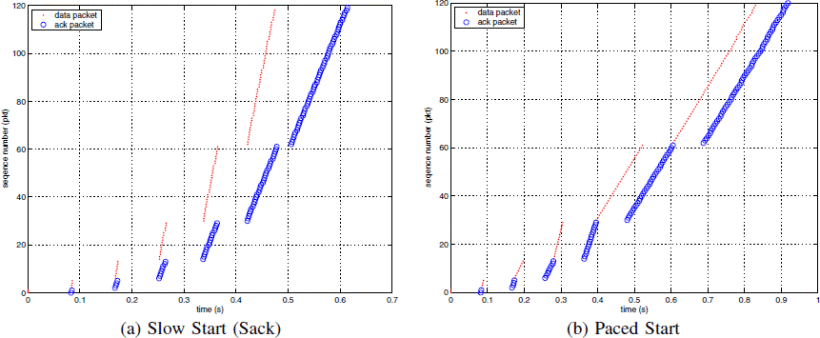
\includegraphics[width=0.5\textwidth]{images/hu03_PTR.png}
	\caption{Figure by Hu et al.~\cite{Hu03}. Packet trains of source and target machines plotted against time for both slow start and paced start algorithm. The data is from a simulation with roundtrip time of 80ms, a bottleneck link of 5Mb/s and available bandwidth of 3Mb/s. In plot (b), the difference of the inter-packet-gaps of the packet trains from source and the target machines converges, yielding the estimate for the available bandwidth. This convergence is visualised in the slopes of the blue and red lines becoming equal.}
	\label{fig:PTR}
\end{figure}
The paced start algorithm is based on the insight, that the TCP startup, with minor changes, can be viewed as a sequence of packet trains, making the PTR method applicable~\cite{Hu03}. The paced start algorithm has two major differences to the slow start algorithm. First, the paced start algorithm is not self clocking (arrival of an ACK does not trigger the sending of packages), because in a self clocking setup the sent and received packets are not even close to being evenly paced, making the inter-packet-gap meaningless to measure. Instead, the paced start only sends a new packet train after the previous packet train has been entirely acknowledged. This allows us to distinguish the packet trains from one another. 

Secondly, paced start iteratively searches for the optimal packet sending rate using the PTR method. The algorithm terminates when a packet is lost or a timeout occurs, just like slow start but also if a sufficiently good packet sending rate is found. Figure~\ref{fig:PTR}, by Ningning Hu and P. Steenkiste~\cite{Hu03}, illustrates the workings of the PTR method.

The paced start algorithm can be described as follows:
\begin{enumerate}
	\item Set \textit{source\_gap} to 0 and \textit{congestion\_window\_size} to 2.
	\item Send \textit{congestion\_window\_size} packets with \textit{source\_gap} and measure \textit{ack\_gap}
	\item Set \textit{source\_gap} to $2 \textit{ack\_gap}$
	\item Double \textit{congestion\_window\_size}, send \textit{congestion\_window\_size} packets with \textit{source\_gap} and measure \textit{ack\_gap}
	\item If packet loss or timeout occurs, start congestion avoidance
	\item If $\textit{src\_gap} - \textit{ack\_gap} \approx 0$, send \textit{congestion\_window\_size} packages and start congestion avoidance, else goto 7
	\item Adjust \textit{source\_gap} based on \textit{ack\_gap} and goto 4 
\end{enumerate} 
The adjustment to \textit{source\_gap} on step 7 is based on the binary search algorithm: if the \textit{source\_gap} is smaller than the measured \textit{ack\_gap}, then we are sending packets at a rate higher than the available rate, and the \textit{source\_gap} must be increased. New \textit{source\_gap} is set to is set to the middle point between measured \textit{ack\_gap} and current upper bound on \textit{source\_gap}.

If \textit{source\_gap} is smaller than the \textit{ack\_gap}, we are sending packets at a lower rate than what is available and the \textit{source\_gap} must be lowered. The \textit{source\_gap} is set to the middle point between previous \textit{source\_gap} and the current lower bound on \textit{source\_gap}.

Figure \ref{fig:paced_start}, by Ningning Hu and P. Steenkiste~\cite{Hu03}, illustrates the bandwidth search functionality of paced start algorithm in the two-dimensional space of sending rate (Y-axis) and train length (X-axis).

\begin{figure}
	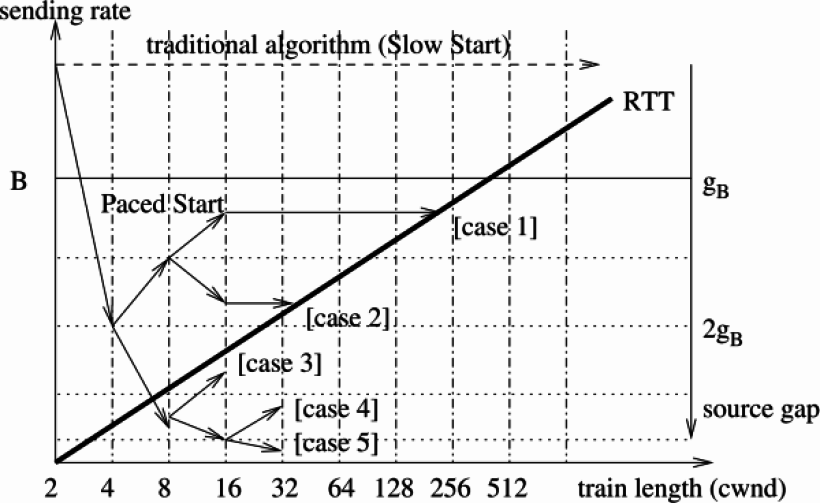
\includegraphics[width=0.5\textwidth]{images/hu03_paced_start_search.png}
	\caption{Figure by Hu et al.~\cite{Hu03}. Slow start algorithm moves along the X-axis until a suitably large cwnd is found (or ssthresh is hit). Paced start also considers the Y-axis, doing a binary search to find the suitable sending rate. Cases 1 to 5 represent possible routes that the binary search may take, depending on the ideal sending rate.}
	\label{fig:paced_start}
\end{figure}

Hu and Steenkiste used ns2 simulator~\cite{Singh12} and real system measurements to evaluate the paced start algorithm, comparing it against the slow start algorithm and TCP Vegas and TCP NewReno, both of which implement their own improvements on the TCP startup algorithm. We well omit the comparison to Vegas and NewReno here and focus solely on the comparison between slow start and paced start. We also omit the large scale network simulation here, reviewing only small scale simulations and system measurements.

Hu and Steenkiste used the following metrics: \textit{throughput} (throughput of the whole connection),  \textit{loss} (loss rate of the whole connection), \textit{su-throughput} (throughput of the startup period), \textit{su-loss} (loss rate of the startup period) and \textit{su-time} (start up period length).  

In the simulation, node \textit{A} initiates a TCP connection to node \textit{B}. The traffic goes through a path that has two routers \textit{$R_1$} and \textit{$R_2$} in between the nodes. Node \textit{A} is connected to \textit{$R_1$} by a fast low latency connection, as is \textit{B} to \textit{$R_2$}. 

The connection between \textit{$R_1$} and \textit{$R_2$} is set at 100Mbps, while the competing traffic load that goes through routers \textit{$R_1$} and \textit{$R_2$} is varied. Metrics \textit{throughput}, \textit{su-throughput}, \textit{loss} and \textit{su-time} are measured, comparing slow start to paced start. The measurements lasted for 50 seconds. Figure~\ref{fig:competing_traffic}, by Ningning Hu and P. Steenkiste~\cite{Hu03}, compiles these measurements.

The lowermost plot clearly shows that paced start moves to congestion avoidance faster than slow start in this scenario. The difference in startup times grows smaller as the amount of competing traffic increases, since slow start requires less and less round trips to find a suitable congestion window.

The plot in the middle shows that paced start algorithm did not lose any packets in this simulation while slow start's loss rate increased as a function of competing traffic. 

The uppermost plot shows that both slow start and paced start achieved roughly the same throughput over the time period of 50 seconds. Paced start performed somewhat better than slow start when little competing traffic was present. This is because in this case, the paced start is able to move to congestion avoidance much faster than slow start. 

Overall, the paced start seems to perform very well compared to slow start in this setup: it is clearly less aggressive, finds a suitable congestion window faster and even has a slight positive impact on the overall throughput.

\begin{figure}
	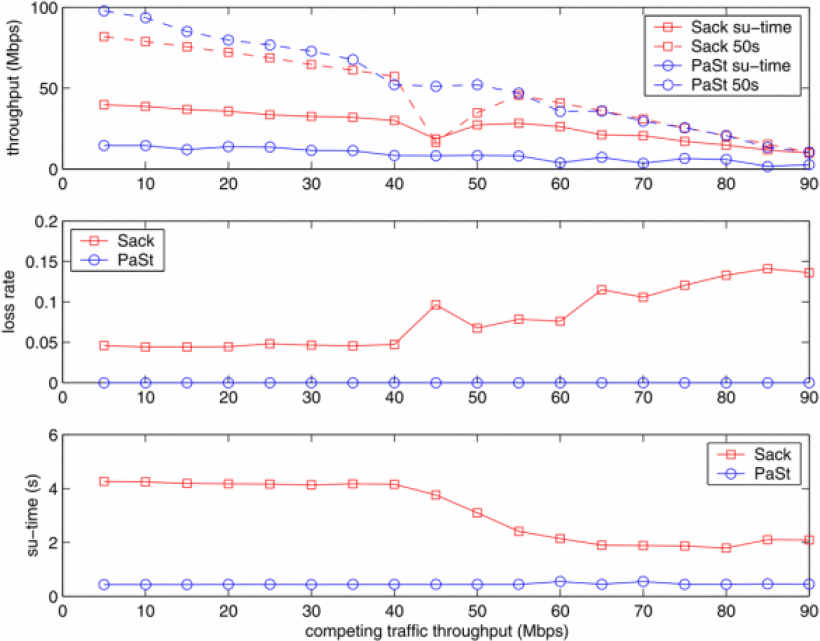
\includegraphics[width=0.5\textwidth]{images/hu03_competing_traffic.png}
	\caption{Figure by Hu et al.~\cite{Hu03}. The effect of competing traffic on the performance of slow start (Sack) and paced start (PaSt) algorithms. ns2 network simulation.}
	\label{fig:competing_traffic}
\end{figure}

A number of experiments were conducted using in-kernel implementation of paced start. The environment was a testbed on Emulab~\cite{Emulab} consisting of two Apache servers and two web request generators, one of each on each side of a bottleneck link, so that bidirectional traffic was generated over the bottleneck link. One of the web servers was configured to use the paced start -kernel while all other hosts used the slow start kernel. The experiments lasted for 500 seconds, each generating around 2100 requests. The web request generators' log files were used to calculate the throughput distribution for downloading web pages. Figure~\ref{fig:in_kernel} contains the throughput distributions, as a CDFs (cumulative distribution functions), of both Apache servers. The web server using paced start lost 1168 packets during the experiment while the web server using slow start lost 94186 packets. The trend of this experiment seems to be similar to that of the simulation: paced start seems to be outperforming slow start in both throughput and packet loss rate.

\begin{figure}
	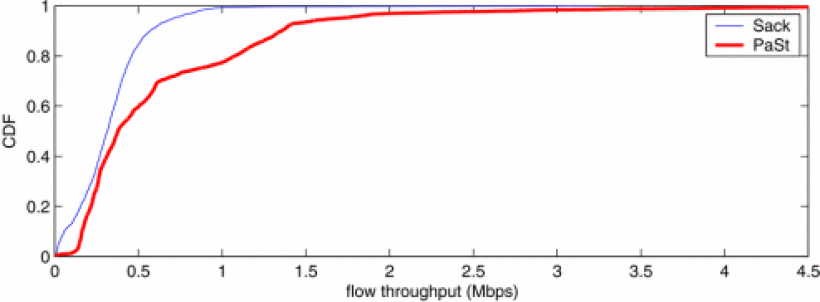
\includegraphics[width=0.5\textwidth]{images/hu03_in_kernel.png}
	\caption{Figure by Hu et al.~\cite{Hu03}. Cumulative distribution functions of flow throughput during a 500 second experiment conducted on a Emulab testbed. Paced start in red and slow start in blue.}
	\label{fig:in_kernel}
\end{figure}



%the difference between the spacing in the data packets and the acknowledgement packets is used to infer information about the bandwidth of the route.


%Alternatively this subsection could be a separate section.